\chapter{Theory}\label{ch:theory}
Here is the theory.

\begin{table}[]
\centering
\caption{The beginnings of the Golomb and Rice codes for a few parameter values. The midpoint ($\cdot$) separates the high-order (unary) part from the low-order (binary) part of the codewords. The codes can be extended to all values of $n\geq0$.}
\label{table:golomb-rice}
\begin{tabular}{rrrrr}
\multicolumn{1}{c}{Golomb}   & \multicolumn{1}{c}{$m=1$}   & \multicolumn{1}{c}{$m=2$}   & \multicolumn{1}{c}{$m=4$}   & \multicolumn{1}{c}{$m=8$}   \\
\multicolumn{1}{c}{Rice}     & \multicolumn{1}{c}{$k=0$}   & \multicolumn{1}{c}{$k=1$}   & \multicolumn{1}{c}{$k=2$}   & \multicolumn{1}{c}{$k=3$}   \\
\hline % --------------------------------------------------------------------------------------------------------------------------------------------
\multicolumn{1}{r|}{$n=0$}   & \textbf{0$\cdot$}           & \textbf{0$\cdot$0}          & \textbf{0$\cdot$00}         & \textbf{0$\cdot$000}        \\
\multicolumn{1}{r|}{      1} & \textbf{10$\cdot$}          & \textbf{0$\cdot$1}          & \textbf{0$\cdot$01}         & \textbf{0$\cdot$001}        \\
\multicolumn{1}{r|}{      2} & \textbf{110$\cdot$}         & \textbf{10$\cdot$0}         & \textbf{0$\cdot$10}         & \textbf{0$\cdot$010}        \\
\multicolumn{1}{r|}{      3} & \textbf{1110$\cdot$}        & \textbf{10$\cdot$1}         & \textbf{0$\cdot$11}         & \textbf{0$\cdot$011}        \\
\multicolumn{1}{r|}{      4} & \textbf{11110$\cdot$}       & \textbf{110$\cdot$0}        & \textbf{10$\cdot$00}        & \textbf{0$\cdot$100}        \\
\multicolumn{1}{r|}{      5} & \textbf{111110$\cdot$}      & \textbf{110$\cdot$1}        & \textbf{10$\cdot$01}        & \textbf{0$\cdot$101}        \\
\multicolumn{1}{r|}{      6} & \textbf{1111110$\cdot$}     & \textbf{1110$\cdot$0}       & \textbf{10$\cdot$10}        & \textbf{0$\cdot$110}        \\
\multicolumn{1}{r|}{      7} & \textbf{11111110$\cdot$}    & \textbf{1110$\cdot$1}       & \textbf{10$\cdot$11}        & \textbf{0$\cdot$111}        \\
\multicolumn{1}{r|}{      8} & \textbf{111111110$\cdot$}   & \textbf{11110$\cdot$0}      & \textbf{110$\cdot$00}       & \textbf{10$\cdot$000}       \\
\multicolumn{1}{r|}{      9} & \textbf{1111111110$\cdot$}  & \textbf{11110$\cdot$1}      & \textbf{110$\cdot$01}       & \textbf{10$\cdot$001}       \\
\multicolumn{1}{r|}{ \vdots} & \multicolumn{1}{c}{\vdots}  & \multicolumn{1}{c}{\vdots}  & \multicolumn{1}{c}{\vdots}  & \multicolumn{1}{c}{\vdots} 
\end{tabular}
\end{table}

\begin{figure}
\centering
\begin{subfigure}[b]{.3\textwidth}
  \centering
  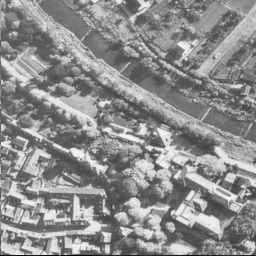
\includegraphics[width=0.95\textwidth]{figures/test-images/original/aerial}
  \caption{Aerial}
  \label{fig:test-images-aerial}
\end{subfigure}
\begin{subfigure}[b]{.3\textwidth}
  \centering
  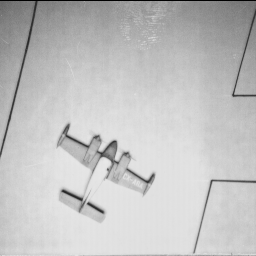
\includegraphics[width=0.95\textwidth]{figures/test-images/original/airplane}
  \caption{Airplane}
  \label{fig:test-images-airplane}
\end{subfigure}
\begin{subfigure}[b]{.3\textwidth}
  \centering
  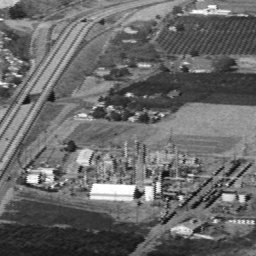
\includegraphics[width=0.95\textwidth]{figures/test-images/original/chemicalplant}
  \caption{Chemical plant }
  \label{fig:test-images-chemicalplant}
\end{subfigure}
\begin{subfigure}[b]{.3\textwidth}
  \centering
  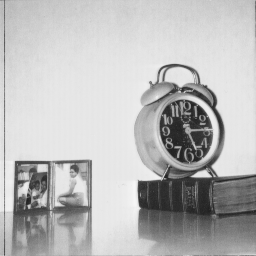
\includegraphics[width=0.95\textwidth]{figures/test-images/original/clock}
  \caption{Clock}
  \label{fig:test-images-clock}
\end{subfigure}
\begin{subfigure}[b]{.3\textwidth}
  \centering
  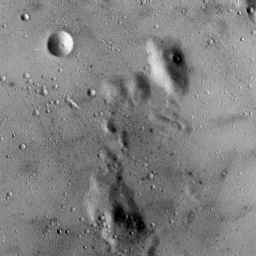
\includegraphics[width=0.95\textwidth]{figures/test-images/original/moonsurface}
  \caption{Moon surface}
  \label{fig:test-images-moonsurface}
\end{subfigure}
\begin{subfigure}[b]{.3\textwidth}
  \centering
  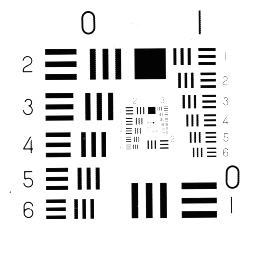
\includegraphics[width=0.95\textwidth]{figures/test-images/original/resolutionchart}
  \caption{Resolution chart}
  \label{fig:test-images-resolutionchart}
\end{subfigure}
\caption{256x256 pixel 8-bits grayscale test images \cite{USC:SIPI}}
\label{fig:test-images}
\end{figure}




\begin{figure}
\centering
\begin{subfigure}[b]{.23\textwidth}
  \centering
  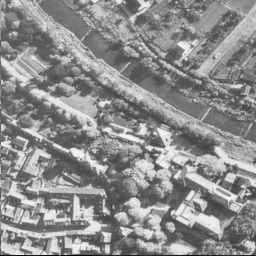
\includegraphics[width=0.95\textwidth]{figures/test-images/original/aerial}
  \caption{Aerial}
  \label{fig:test-images-aerial-original}
\end{subfigure}
\begin{subfigure}[b]{.23\textwidth}
  \centering
  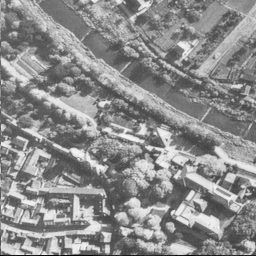
\includegraphics[width=0.95\textwidth]{figures/test-images/truncate1/aerial}
  \caption{}
  \label{fig:test-images-aerial-truncate1}
\end{subfigure}
\begin{subfigure}[b]{.23\textwidth}
  \centering
  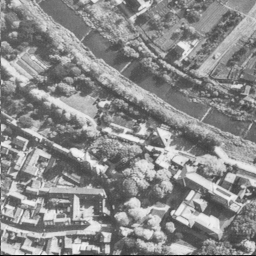
\includegraphics[width=0.95\textwidth]{figures/test-images/truncate2/aerial}
  \caption{}
  \label{fig:test-images-aerial-truncate2}
\end{subfigure}
\begin{subfigure}[b]{.23\textwidth}
  \centering
  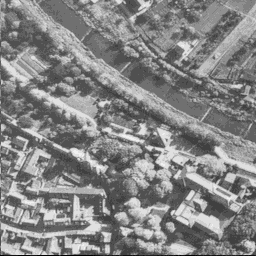
\includegraphics[width=0.95\textwidth]{figures/test-images/truncate4/aerial}
  \caption{}
  \label{fig:test-images-aerial-truncate4}
\end{subfigure}

\begin{subfigure}[b]{.23\textwidth}
  \centering
  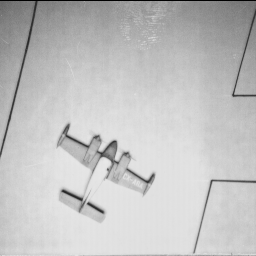
\includegraphics[width=0.95\textwidth]{figures/test-images/original/airplane}
  \caption{Airplane}
  \label{fig:test-images-airplane-original}
\end{subfigure}
\begin{subfigure}[b]{.23\textwidth}
  \centering
  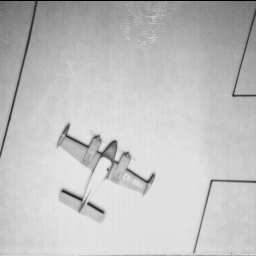
\includegraphics[width=0.95\textwidth]{figures/test-images/truncate1/airplane}
  \caption{}
  \label{fig:test-images-airplane-truncate1}
\end{subfigure}
\begin{subfigure}[b]{.23\textwidth}
  \centering
  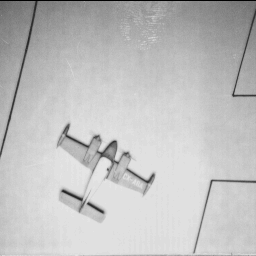
\includegraphics[width=0.95\textwidth]{figures/test-images/truncate2/airplane}
  \caption{}
  \label{fig:test-images-airplane-truncate2}
\end{subfigure}
\begin{subfigure}[b]{.23\textwidth}
  \centering
  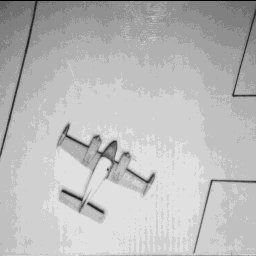
\includegraphics[width=0.95\textwidth]{figures/test-images/truncate4/airplane}
  \caption{}
  \label{fig:test-images-airplane-truncate4}
\end{subfigure}

\begin{subfigure}[b]{.23\textwidth}
  \centering
  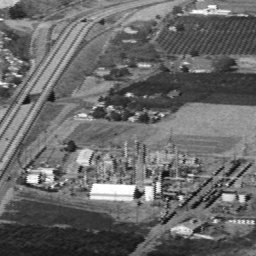
\includegraphics[width=0.95\textwidth]{figures/test-images/original/chemicalplant}
  \caption{Chemical plant}
  \label{fig:test-images-chemicalplant-original}
\end{subfigure}
\begin{subfigure}[b]{.23\textwidth}
  \centering
  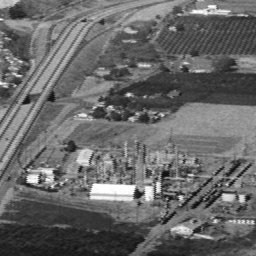
\includegraphics[width=0.95\textwidth]{figures/test-images/truncate1/chemicalplant}
  \caption{}
  \label{fig:test-images-chemicalplant-truncate1}
\end{subfigure}
\begin{subfigure}[b]{.23\textwidth}
  \centering
  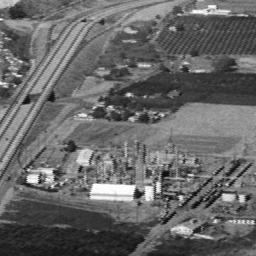
\includegraphics[width=0.95\textwidth]{figures/test-images/truncate2/chemicalplant}
  \caption{}
  \label{fig:test-images-chemicalplant-truncate2}
\end{subfigure}
\begin{subfigure}[b]{.23\textwidth}
  \centering
  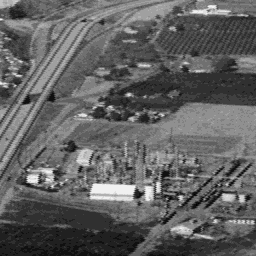
\includegraphics[width=0.95\textwidth]{figures/test-images/truncate4/chemicalplant}
  \caption{}
  \label{fig:test-images-chemicalplant-truncate4}
\end{subfigure}

\begin{subfigure}[b]{.23\textwidth}
  \centering
  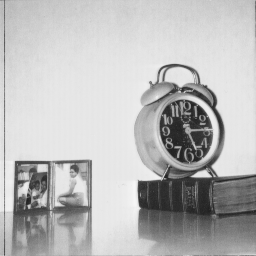
\includegraphics[width=0.95\textwidth]{figures/test-images/original/clock}
  \caption{Clock}
  \label{fig:test-images-clock-original}
\end{subfigure}
\begin{subfigure}[b]{.23\textwidth}
  \centering
  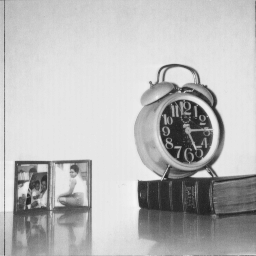
\includegraphics[width=0.95\textwidth]{figures/test-images/truncate1/clock}
  \caption{}
  \label{fig:test-images-clock-truncate1}
\end{subfigure}
\begin{subfigure}[b]{.23\textwidth}
  \centering
  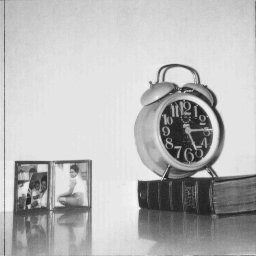
\includegraphics[width=0.95\textwidth]{figures/test-images/truncate2/clock}
  \caption{}
  \label{fig:test-images-clock-truncate2}
\end{subfigure}
\begin{subfigure}[b]{.23\textwidth}
  \centering
  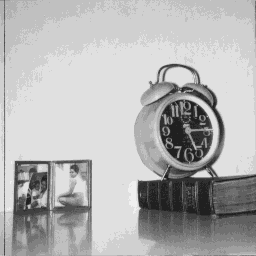
\includegraphics[width=0.95\textwidth]{figures/test-images/truncate4/clock}
  \caption{}
  \label{fig:test-images-clock-truncate4}
\end{subfigure}

\begin{subfigure}[b]{.23\textwidth}
  \centering
  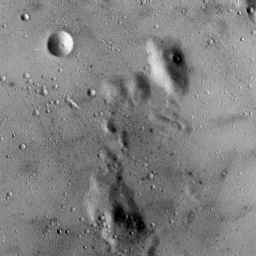
\includegraphics[width=0.95\textwidth]{figures/test-images/original/moonsurface}
  \caption{Moon surface}
  \label{fig:test-images-moonsurface-original}
\end{subfigure}
\begin{subfigure}[b]{.23\textwidth}
  \centering
  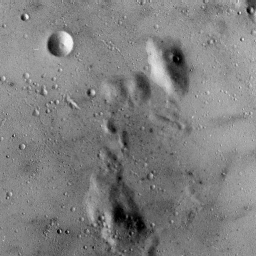
\includegraphics[width=0.95\textwidth]{figures/test-images/truncate1/moonsurface}
  \caption{}
  \label{fig:test-images-moonsurface-truncate1}
\end{subfigure}
\begin{subfigure}[b]{.23\textwidth}
  \centering
  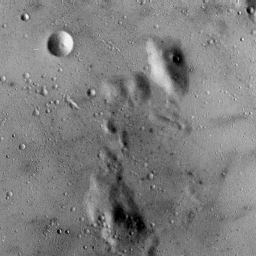
\includegraphics[width=0.95\textwidth]{figures/test-images/truncate2/moonsurface}
  \caption{}
  \label{fig:test-images-moonsurface-truncate2}
\end{subfigure}
\begin{subfigure}[b]{.23\textwidth}
  \centering
  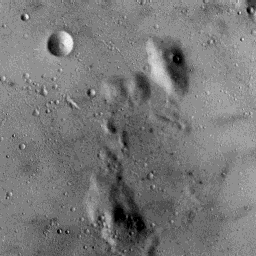
\includegraphics[width=0.95\textwidth]{figures/test-images/truncate4/moonsurface}
  \caption{}
  \label{fig:test-images-moonsurface-truncate4}
\end{subfigure}

\begin{subfigure}[b]{.23\textwidth}
  \centering
  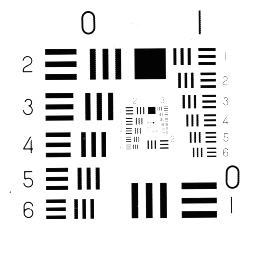
\includegraphics[width=0.95\textwidth]{figures/test-images/original/resolutionchart}
  \caption{Res. chart}
  \label{fig:test-images-resolutionchart-original}
\end{subfigure}
\begin{subfigure}[b]{.23\textwidth}
  \centering
  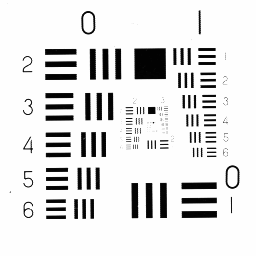
\includegraphics[width=0.95\textwidth]{figures/test-images/truncate1/resolutionchart}
  \caption{}
  \label{fig:test-images-resolutionchart-truncate1}
\end{subfigure}
\begin{subfigure}[b]{.23\textwidth}
  \centering
  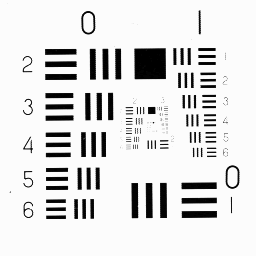
\includegraphics[width=0.95\textwidth]{figures/test-images/truncate2/resolutionchart}
  \caption{}
  \label{fig:test-images-resolutionchart-truncate2}
\end{subfigure}
\begin{subfigure}[b]{.23\textwidth}
  \centering
  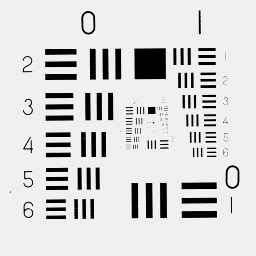
\includegraphics[width=0.95\textwidth]{figures/test-images/truncate4/resolutionchart}
  \caption{}
  \label{fig:test-images-resolutionchart-truncate4}
\end{subfigure}
\caption{Restored images after lossy compression. Left pictures are the originals, right of then are the results of the Truncate1 compresseion, then Truncate2 and on the right Truncate4.}
\label{fig:test-images-restored}
\end{figure}


\begin{figure}[htbp]
    \centering
    \begin{subfigure}[t]{0.3\textwidth}\tightdisplaymath
        \centerline{
        \xymatrix@ = 2pt{
            a_7 & a_6 & a_5 & a_4 & a_3 & a_2 & a_1 & a_0 \\
            b_7 & b_6 & b_5 & b_4 & b_3 & b_2 & b_1 & b_0 \\
            c_7 & c_6 & c_5 & c_4 & c_3 & c_2 & c_1 & c_0 \\
            d_7 & d_6 & d_5 & d_4 & d_3 & d_2 & d_1 & d_0 \\
            e_7 & e_6 & e_5 & e_4 & e_3 & e_2 & e_1 & e_0 \\
            f_7 & f_6 & f_5 & f_4 & f_3 & f_2 & f_1 & f_0 \\
            g_7 & g_6 & g_5 & g_4 & g_3 & g_2 & g_1 & g_0 \\
            h_7 & h_6 & h_5 & h_4 & h_3 & h_2 & h_1 & h_0 }}
        \caption{8 uncompressed bytes.}
    \end{subfigure}
    \hspace*{3cm}
    \begin{subfigure}[t]{0.3\textwidth}\tightdisplaymath
        \centerline{
        \xymatrix@=2pt{
            a_7 & a_6 & a_5 & a_4 & a_3 & a_2 & a_1 & \_ \\
            b_7 & b_6 & b_5 & b_4 & b_3 & b_2 & b_1 & \_ \\
            c_7 & c_6 & c_5 & c_4 & c_3 & c_2 & c_1 & \_ \\
            d_7 & d_6 & d_5 & d_4 & d_3 & d_2 & d_1 & \_ \\
            e_7 & e_6 & e_5 & e_4 & e_3 & e_2 & e_1 & \_ \\
            f_7 & f_6 & f_5 & f_4 & f_3 & f_2 & f_1 & \_ \\
            g_7 & g_6 & g_5 & g_4 & g_3 & g_2 & g_1 & \_ \\
            h_7 \ar[urrrrrrr] & h_6\ar[uurrrrrr] & h_5 \ar[uuurrrrr]& h_4 \ar[uuuurrrr] & h_3 \ar[uuuuurrr] & h_2 \ar[uuuuuurr] & h_1 \ar[uuuuuuur] & \_ }}
            \caption{Compressing 8 to 7 bytes.}
    \end{subfigure}
    \begin{subfigure}[t]{0.3\textwidth}\tightdisplaymath
        \centerline{
        \xymatrix@ = 2pt{
            a_7 & a_6 & a_5 & a_4 & a_3 & a_2 & a_1 & h_1 \\
            b_7 & b_6 & b_5 & b_4 & b_3 & b_2 & b_1 & h_2 \\
            c_7 & c_6 & c_5 & c_4 & c_3 & c_2 & c_1 & h_3 \\
            d_7 & d_6 & d_5 & d_4 & d_3 & d_2 & d_1 & h_4 \\
            e_7 & e_6 & e_5 & e_4 & e_3 & e_2 & e_1 & h_5 \\
            f_7 & f_6 & f_5 & f_4 & f_3 & f_2 & f_1 & h_6 \\
            g_7 & g_6 & g_5 & g_4 & g_3 & g_2 & g_1 & h_7 }}
        \caption{7 compressed bytes.}
    \end{subfigure}
    \caption{Truncate1 compression algorithm.}
    \label{fig:truncate1-compression-algo}
\end{figure}

\begin{figure}[htbp]
    \centering
    \begin{subfigure}[t]{0.3\textwidth}\tightdisplaymath
        \centerline{
        \xymatrix@ = 2pt{
            a_7 & a_6 & a_5 & a_4 & a_3 & a_2 & a_1 & a_0 \\
            b_7 & b_6 & b_5 & b_4 & b_3 & b_2 & b_1 & b_0 \\
            c_7 & c_6 & c_5 & c_4 & c_3 & c_2 & c_1 & c_0 \\
            d_7 & d_6 & d_5 & d_4 & d_3 & d_2 & d_1 & d_0 }}
        \caption{4 uncompressed bytes.}
    \end{subfigure}
    \hspace*{3cm}
    \begin{subfigure}[t]{0.3\textwidth}\tightdisplaymath
        \centerline{
        \xymatrix@=2pt{
            a_7 & a_6 & a_5 & a_4 & a_3 & a_2 & \_ & \_ \\
            b_7 & b_6 & b_5 & b_4 & b_3 & b_2 & \_ & \_ \\
            c_7 & c_6 & c_5 & c_4 & c_3 & c_2 & \_ & \_ \\
            d_7 \ar[urrrrrr] & d_6\ar[urrrrrr] & d_5 \ar[uurrrr]& d_4 \ar[uurrrr] & d_3 \ar[uuurr] & d_2 \ar[uuurr] & \_ & \_ }}
            \caption{Compressing 4 to 3 bytes.}
    \end{subfigure}
    \begin{subfigure}[t]{0.3\textwidth}\tightdisplaymath
        \centerline{
        \xymatrix@ = 2pt{
            a_7 & a_6 & a_5 & a_4 & a_3 & a_2 & d_3 & d_2 \\
            b_7 & b_6 & b_5 & b_4 & b_3 & b_2 & d_5 & d_4 \\
            c_7 & c_6 & c_5 & c_4 & c_3 & c_2 & d_7 & d_6 }}
        \caption{3 compressed bytes.}
    \end{subfigure}
    \caption{Truncate2 compression algorithm.}
    \label{fig:truncate2-compression-algo}
\end{figure}

\begin{figure}[htbp]
    \centering
    \begin{subfigure}[t]{0.3\textwidth}\tightdisplaymath
        \centerline{
        \xymatrix@ = 2pt{
            a_7 & a_6 & a_5 & a_4 & a_3 & a_2 & a_1 & a_0 \\
            b_7 & b_6 & b_5 & b_4 & b_3 & b_2 & b_1 & b_0 }}
        \caption{2 uncompressed bytes.}
    \end{subfigure}
    \hspace*{3cm}
    \begin{subfigure}[t]{0.3\textwidth}\tightdisplaymath
        \centerline{
        \xymatrix@=2pt{
            a_7 & a_6 & a_5 & a_4 & \_ & \_ & \_ & \_ \\
            b_7 \ar[urrrr] & b_6\ar[urrrr] & b_5 \ar[urrrr]& b_4 \ar[urrrr] & \_ & \_ & \_ & \_ }}
            \caption{Compressing 2 to 1 bytes.}
    \end{subfigure}
    \begin{subfigure}[t]{0.3\textwidth}\tightdisplaymath
        \centerline{
        \xymatrix@ = 2pt{
            a_7 & a_6 & a_5 & a_4 & b_7 & b_6 & b_5 & b_4 }}
        \caption{1 compressed bytes.}
    \end{subfigure}
    \caption{Truncate4 compression algorithm.}
    \label{fig:truncate4-compression-algo}
\end{figure}



